\documentclass[article]{jss}
\usepackage{booktabs}

%%%%%%%%%%%%%%%%%%%%%%%%%%%%%%
%% declarations for jss.cls %%%%%%%%%%%%%%%%%%%%%%%%%%%%%%%%%%%%%%%%%%
%%%%%%%%%%%%%%%%%%%%%%%%%%%%%%

%
% Local helpers to make this more compatible with R Journal style.
%
\newcommand{\CRANpkg}[1]{\pkg{#1}}
\RequirePackage{fancyvrb}
\RequirePackage{alltt}
\DefineVerbatimEnvironment{example}{Verbatim}{}

%% almost as usual
\author{Dirk Eddelbuettel\\Debian and R Projects \And 
        Murray Stokely\\Google, Inc}
\title{\pkg{RProtoBuf}: Efficient Cross-Language Data Serialization in R}

%% for pretty printing and a nice hypersummary also set:
\Plainauthor{Dirk Eddelbuettel, Murray Stokely} %% comma-separated
\Plaintitle{RProtoBuf: Efficient Cross-Language Data Serialization in R}
\Shorttitle{\pkg{RProtoBuf}: Protocol Buffers in R} %% a short title (if necessary)

%% an abstract and keywords
\Abstract{
Modern data collection and analysis pipelines often involve
a sophisticated mix of applications written in general purpose and
specialized programming languages.  Protocol Buffers are a popular
method of serializing structured data between applications---while remaining
independent of programming languages or operating system.  The
\CRANpkg{RProtoBuf} package provides a complete interface to this
library.
}
\Keywords{r, protocol buffers, serialization, cross-platform}
\Plainkeywords{r, protocol buffers, serialization, cross-platform} %% without formatting
%% at least one keyword must be supplied

%% publication information
%% NOTE: Typically, this can be left commented and will be filled out by the technical editor
%% \Volume{50}
%% \Issue{9}
%% \Month{June}
%% \Year{2012}
%% \Submitdate{2012-06-04}
%% \Acceptdate{2012-06-04}

%% The address of (at least) one author should be given
%% in the following format:
\Address{
  Dirk Eddelbuettel\\
  \\
  Murray Stokely\\
  Google, Inc.\\
  1600 Amphitheatre Parkway\\
  Mountain View, CA 94040\\
  USA\\
  E-mail: \email{mstokely@google.com}\\
  URL: \url{http://www.stokely.org/}
}
%% It is also possible to add a telephone and fax number
%% before the e-mail in the following format:
%% Telephone: +43/512/507-7103
%% Fax: +43/512/507-2851

%% for those who use Sweave please include the following line (with % symbols):
%% need no \usepackage{Sweave.sty}

%% end of declarations %%%%%%%%%%%%%%%%%%%%%%%%%%%%%%%%%%%%%%%%%%%%%%%


\begin{document}


%% include your article here, just as usual
%% Note that you should use the \pkg{}, \proglang{} and \code{} commands.


% We don't want a left margin for Sinput or Soutput for our table 1.
%\DefineVerbatimEnvironment{Sinput}{Verbatim} {xleftmargin=0em}
%\DefineVerbatimEnvironment{Soutput}{Verbatim}{xleftmargin=0em}
%\DefineVerbatimEnvironment{Scode}{Verbatim}{xleftmargin=2em}
% Setting the topsep to 0 reduces spacing from input to output and
% improves table 1.
\fvset{listparameters={\setlength{\topsep}{0pt}}}
\renewenvironment{Schunk}{\vspace{\topsep}}{\vspace{\topsep}}

\title{RProtoBuf: Efficient Cross-Language Data Serialization in R}
\author{by Dirk Eddelbuettel and Murray Stokely}

%% DE: I tend to have wider option(width=...) so this
%%     guarantees better line breaks

\maketitle

\abstract{Modern data collection and analysis pipelines often involve
 a sophisticated mix of applications written in general purpose and
 specialized programming languages.  Protocol Buffers are a popular
 method of serializing structured data between applications---while remaining
 independent of programming languages or operating system.  The
 \CRANpkg{RProtoBuf} package provides a complete interface between this
 library and the R environment for statistical computing.
 %TODO(ms) keep it less than 150 words.
}

%TODO(de) 'protocol buffers' or 'Protocol Buffers' ?

\section{Introduction}

Modern data collection and analysis pipelines are increasingly being
built using collections of components to better manage software
complexity through reusability, modularity, and fault
isolation \citep{Wegiel:2010:CTT:1932682.1869479}.
Data analysis patterns such as Split-Apply-Combine
\citep{wickham2011split} explicitly break up large problems into
manageable pieces.  These patterns are frequently employed with
different programming languages used for the different phases of data
analysis -- collection, cleaning, analysis, post-processing, and
presentation in order to take advantage of the unique combination of
performance, speed of development, and library support offered by
different environments.  Each stage of the data
analysis pipeline may involve storing intermediate results in a
file or sending them over the network.
% DE: Nice!

Given these requirements, how do we safely share intermediate results
between different applications, possibly written in different
languages, and possibly running on different computer system, possibly
spanning different operating systems?  Programming
languages such as R, Julia, Java, and Python include built-in
serialization support, but these formats are tied to the specific
% DE: need to define serialization?
programming language in use and thus lock the user into a single
environment.  CSV files can be read and written by many applications
and so are often used for exporting tabular data.  However, CSV files
have a number of disadvantages, such as a limitation of exporting only
tabular datasets, lack of type-safety, inefficient text representation
and parsing, and ambiguities in the format involving special
characters.  JSON is another widely-supported format used mostly on
the web that removes many of these disadvantages, but it too suffers
from being too slow to parse and also does not provide strong typing
between integers and floating point.  Because the schema information
is not kept separately, multiple JSON messages of the same type
needlessly duplicate the field names with each message.
%
%
%
A number of binary formats based on JSON have been proposed that
reduce the parsing cost and improve the efficiency.  MessagePack
\citep{msgpackR} and BSON \citep{rmongodb} both have R interfaces, but
these formats lack a separate schema for the serialized data and thus
still duplicate field names with each message sent over the network or
stored in a file.  Such formats also lack support for versioning when
data storage needs evolve over time, or when application logic and
requirement changes dictate update to the message format.
% DE: Need to talk about XML ?

Once the data serialization needs of an application become complex
enough, developers typically benefit from the use of an
\emph{interface description language}, or \emph{IDL}.  IDLs like
Protocol Buffers \citep{protobuf}, Apache Thrift, and Apache Avro provide a compact
well-documented schema for cross-langauge data structures and
efficient binary interchange formats.  The schema can be used to
generate model classes for statically-typed programming languages such
as C++ and Java, or can be used with reflection for dynamically-typed
programming languages.  Since the schema is provided separately from
the encoded data, the data can be efficiently encoded to minimize
storage costs of the stored data when compared with simple
``schema-less'' binary interchange formats.

% TODO(mstokely): Take a more conversational tone here asking
% questions and motivating protocol buffers?

% TODO(mstokely): If we go to JSS, include a larger paragraph here
% referencing each numbered section.  I don't like these generally,
% but its useful for this paper I think because we have a boring bit
% in the middle (full class/method details) and interesting
% applications at the end.
This article describes the basics of Google's Protocol Buffers through
an easy to use R package, \CRANpkg{RProtoBuf}.  After describing the
basics of protocol buffers and \CRANpkg{RProtoBuf}, we illustrate
several common use cases for protocol buffers in data analysis.

\section{Protocol Buffers}

FIXME Introductory section which may include references in parentheses
\citep{R}, or cite a reference such as \citet{R} in the text.

% This content is good.  Maybe use and cite?
% http://martin.kleppmann.com/2012/12/05/schema-evolution-in-avro-protocol-buffers-thrift.html


%% TODO(de,ms)  What follows is oooooold and was lifted from the webpage
%%              Rewrite?
Protocol Buffers can be described as a modern, language-neutral, platform-neutral,
extensible mechanism for sharing and storing structured data.  Since their
introduction, Protocol Buffers have been widely adopted in industry with
applications as varied as database-internal messaging (Drizzle), % DE: citation?
Sony Playstations, Twitter, Google Search, Hadoop, and Open Street Map.  While
% TODO(DE): This either needs a citation, or remove the name drop
traditional IDLs have at time been criticized for code bloat and
complexity, Protocol Buffers are based on a simple list and records
model that is compartively flexible and simple to use.

Some of the key features provided by Protocol Buffers for data analysis
include:

\begin{itemize}
\item \emph{Portable}:  Allows users to send and receive data between
  applications or different computers.
\item \emph{Efficient}:  Data is serialized into a compact binary
  representation for transmission or storage.
\item \emph{Exentsible}:  New fields can be added to Protocol Buffer Schemas
  in a forward-compatible way that do not break older applications.
\item \emph{Stable}:  Protocol Buffers have been in wide use for over a
  decade.
\end{itemize}

Figure~\ref{fig:protobuf-distributed-usecase} illustrates an example
communication workflow with protocol buffers and an interactive R
session.  Common use cases include populating a request RPC protocol
buffer in R that is then serialized and sent over the network to a
remote server.  The server would then deserialize the message, act on
the request, and respond with a new protocol buffer over the network. The key
difference to, say, a request to an Rserve instance is that the remote server
may not even know the R language.

%Protocol buffers are a language-neutral, platform-neutral, extensible
%way of serializing structured data for use in communications
%protocols, data storage, and more.

%Protocol Buffers offer key features such as an efficient data interchange
%format that is both language- and operating system-agnostic yet uses a
%lightweight and highly performant encoding, object serialization and
%de-serialization as well data and configuration management. Protocol
%buffers are also forward compatible: updates to the \texttt{proto}
%files do not break programs built against the previous specification.

%While benchmarks are not available, Google states on the project page that in
%comparison to XML, protocol buffers are at the same time \textsl{simpler},
%between three to ten times \textsl{smaller}, between twenty and one hundred
%times \textsl{faster}, as well as less ambiguous and easier to program.

Many sources compare data serialization formats and show protocol
buffers very favorably to the alternatives, such
as \citet{Sumaray:2012:CDS:2184751.2184810}

%The flexibility of the reflection-based API is particularly well
%suited for interactive data analysis.

% XXX Design tradeoffs: reflection vs proto compiler

For added speed and efficiency, the C++, Java, and Python bindings to
Protocol Buffers are used with a compiler that translates a protocol
buffer schema description file (ending in \texttt{.proto}) into
language-specific classes that can be used to create, read, write and
manipulate protocol buffer messages.  The R interface, in contrast,
uses a reflection-based API that is particularly well suited for
interactive data analysis.  All messages in R have a single class
structure, but different accessor methods are created at runtime based
on the name fields of the specified message type.

% In other words, given the 'proto'
%description file, code is automatically generated for the chosen
%target language(s). The project page contains a tutorial for each of
%these officially supported languages:
%\url{http://code.google.com/apis/protocolbuffers/docs/tutorials.html}

%The protocol buffers code is released under an open-source (BSD) license. The
%protocol buffer project (\url{http://code.google.com/p/protobuf/})
%contains a C++ library and a set of runtime libraries and compilers for
%C++, Java and Python.

%With these languages, the workflow follows standard practice of so-called
%Interface Description Languages (IDL)
%(c.f. \href{http://en.wikipedia.org/wiki/Interface_description_language}{Wikipedia
%  on IDL}).  This consists of compiling a protocol buffer description file
%(ending in \texttt{.proto}) into language specific classes that can be used

%Besides the officially supported C++, Java and Python implementations, several projects have been
%created to support protocol buffers for many languages. The list of known
%languages to support protocol buffers is compiled as part of the
%project page: \url{http://code.google.com/p/protobuf/wiki/ThirdPartyAddOns}

\begin{figure}[t]
\begin{center}
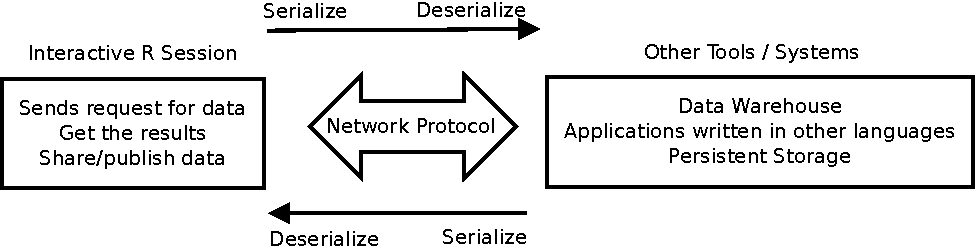
\includegraphics[width=\textwidth]{protobuf-distributed-system-crop.pdf}
\end{center}
\caption{Example protobuf usage}
\label{fig:protobuf-distributed-usecase}
\end{figure}

\section{Basic Usage: Messages and Descriptors}

This section describes how to use the R API to create and manipulate
protocol buffer messages in R, and how to read and write the
binary \emph{payload} of the messages to files and arbitrary binary
R connections.

The two fundamental building blocks of Protocol Buffers are Messages
and Descriptors.  Messages provide a common abstract encapsulation of
structured data fields of the type specified in a Message Descriptor.
Message Descriptors are defined in \texttt{.proto} files and define a
schema for a particular named class of messages.

Table~\ref{tab:proto} shows an example \texttt{.proto} file which
defines the \texttt{tutorial.Person} type.  The R code in the right
column shows an example of creating a new message of this type and
populating its fields.

% Commented out because we said this earlier.
%This separation
%between schema and the message objects is in contrast to
%more verbose formats like JSON, and when combined with the efficient
%binary representation of any Message object explains a large part of
%the performance and storage-space advantage offered by Protocol
%Buffers. TODO(ms): we already said some of this above.  clean up.

% lifted from protobuf page:
%With Protocol Buffers you define how you want your data to be
%structured once, and then you can read or write structured data to and
%from a variety of data streams using a variety of different
%languages.  The definition


%% TODO(de) Can we make this not break the width of the page?
\noindent
\begin{table}
\begin{tabular}{@{\hskip .01\textwidth}p{.40\textwidth}@{\hskip .02\textwidth}@{\hskip .02\textwidth}p{0.55\textwidth}@{\hskip .01\textwidth}}
\toprule
Schema : \texttt{addressbook.proto} & Example R Session\\
\cmidrule{1-2}
\begin{minipage}{.35\textwidth}
\vspace{2mm}
\begin{example}
package tutorial;
message Person {
 required string name = 1;
 required int32 id = 2;
 optional string email = 3;
 enum PhoneType {
   MOBILE = 0; HOME = 1;
   WORK = 2;
 }
 message PhoneNumber {
   required string number = 1;
   optional PhoneType type = 2;
 }
 repeated PhoneNumber phone = 4;
}
\end{example}
\vspace{2mm}
\end{minipage} & \begin{minipage}{.5\textwidth}
\begin{Schunk}
\begin{Sinput}
R> library(RProtoBuf)
R> p <- new(tutorial.Person, id=1, name="Dirk")
R> class(p)
\end{Sinput}
\begin{Soutput}
[1] "Message"
attr(,"package")
[1] "RProtoBuf"
\end{Soutput}
\begin{Sinput}
R> p$name
\end{Sinput}
\begin{Soutput}
[1] "Dirk"
\end{Soutput}
\begin{Sinput}
R> p$name <- "Murray"
R> cat(as.character(p))
\end{Sinput}
\begin{Soutput}
name: "Murray"
id: 1
\end{Soutput}
\begin{Sinput}
R> serialize(p, NULL)
\end{Sinput}
\begin{Soutput}
 [1] 0a 06 4d 75 72 72 61 79 10 01
\end{Soutput}
\end{Schunk}
\end{minipage} \\
\bottomrule
\end{tabular}
\caption{The schema representation from a \texttt{.proto} file for the
  \texttt{tutorial.Person} class (left) and simple R code for creating
  an object of this class and accessing its fields (right).}
\label{tab:proto}
\end{table}

%This section may contain a figure such as Figure~\ref{figure:rlogo}.
%
%\begin{figure}[htbp]
%  \centering
%  \includegraphics{Rlogo}
%  \caption{The logo of R.}
%  \label{figure:rlogo}
%\end{figure}

\subsection{Importing Message Descriptors from .proto files}

%The three basic abstractions of \CRANpkg{RProtoBuf} are Messages,
%which encapsulate a data structure, Descriptors, which define the
%schema used by one or more messages, and DescriptorPools, which
%provide access to descriptors.

Before one can create a new Protocol Buffer Message or parse a
serialized stream of bytes as a Message, one must first read in the message
type specification from a \texttt{.proto} file.

New \texttt{.proto} files are imported with the \code{readProtoFiles}
function, which can import a single file, all files in a directory, or
all \texttt{.proto} files provided by another R package.

The \texttt{.proto} file syntax for defining the structure of protocol
buffer data is described comprehensively on Google Code:
\url{http://code.google.com/apis/protocolbuffers/docs/proto.html}.

Once the proto files are imported, all message descriptors are
are available in the R search path in the \texttt{RProtoBuf:DescriptorPool}
special environment. The underlying mechanism used here is
described in more detail in Section~\ref{sec-lookup}.

\begin{Schunk}
\begin{Sinput}
R> ls("RProtoBuf:DescriptorPool")
\end{Sinput}
\begin{Soutput}
 [1] "rexp.CMPLX"                  
 [2] "rexp.REXP"                   
 [3] "rexp.STRING"                 
 [4] "rprotobuf.HelloWorldRequest" 
 [5] "rprotobuf.HelloWorldResponse"
 [6] "tutorial.AddressBook"        
 [7] "tutorial.Person"             
 [8] "tutorial.Test1"              
 [9] "tutorial.Test2"              
[10] "tutorial.Test3"              
[11] "tutorial.Test4"              
\end{Soutput}
\end{Schunk}

%\subsection{Importing proto files}
%In contrast to the other languages (Java, C++, Python) that are officially
%supported by Google, the implementation used by the \texttt{RProtoBuf}
%package does not rely on the \texttt{protoc} compiler (with the exception of
%the two functions discussed in the previous section). This means that no
%initial step of statically compiling the proto file into C++ code that is
%then accessed by R code is necessary. Instead, \texttt{proto} files are
%parsed and processed \textsl{at runtime} by the protobuf C++ library---which
%is much more appropriate for a dynamic language.

\subsection{Creating a message}

New messages are created with the \texttt{new} function which accepts
a Message Descriptor and optionally a list of ``name = value'' pairs
to set in the message.
%The objects contained in the special environment are
%descriptors for their associated message types. Descriptors will be
%discussed in detail in another part of this document, but for the
%purpose of this section, descriptors are just used with the \texttt{new}
%function to create messages.

\begin{Schunk}
\begin{Sinput}
R> p1 <- new(tutorial.Person)
R> p <- new(tutorial.Person, name = "Murray", id = 1)
\end{Sinput}
\end{Schunk}

\subsection{Access and modify fields of a message}

Once the message is created, its fields can be queried
and modified using the dollar operator of R, making protocol
buffer messages seem like lists.

\begin{Schunk}
\begin{Sinput}
R> p$name
\end{Sinput}
\begin{Soutput}
[1] "Murray"
\end{Soutput}
\begin{Sinput}
R> p$id
\end{Sinput}
\begin{Soutput}
[1] 1
\end{Soutput}
\begin{Sinput}
R> p$email <- "murray@stokely.org"
\end{Sinput}
\end{Schunk}

However, as opposed to R lists, no partial matching is performed
and the name must be given entirely.

The \verb|[[| operator can also be used to query and set fields
of a mesages, supplying either their name or their tag number :

\begin{Schunk}
\begin{Sinput}
R> p[["name"]] <- "Murray Stokely"
R> p[[ 2 ]] <- 3
R> p[[ "email" ]]
\end{Sinput}
\begin{Soutput}
[1] "murray@stokely.org"
\end{Soutput}
\end{Schunk}

Protocol buffers include a 64-bit integer type, but R lacks native
64-bit integer support.  A workaround is available and described in
Section~\ref{sec:int64} for working with large integer values.

% TODO(mstokely): Document extensions here.
% There are none in addressbook.proto though.

\subsection{Display messages}

Protocol buffer messages and descriptors implement \texttt{show}
methods that provide basic information about the message :

\begin{Schunk}
\begin{Sinput}
R> p
\end{Sinput}
\begin{Soutput}
[1] "message of type 'tutorial.Person' with 3 fields set"
\end{Soutput}
\end{Schunk}

For additional information, such as for debugging purposes,
the \texttt{as.character} method provides a more complete ASCII
representation of the contents of a message.

\begin{Schunk}
\begin{Sinput}
R> writeLines(as.character(p))
\end{Sinput}
\begin{Soutput}
name: "Murray Stokely"
id: 3
email: "murray@stokely.org"
\end{Soutput}
\end{Schunk}

\subsection{Serializing messages}

However, the main focus of protocol buffer messages is
efficiency. Therefore, messages are transported as a sequence
of bytes. The \texttt{serialize} method is implemented for
protocol buffer messages to serialize a message into a sequence of
bytes that represents the message.
%(raw vector in R speech) that represents the message.

\begin{Schunk}
\begin{Sinput}
R> serialize(p, NULL)
\end{Sinput}
\begin{Soutput}
 [1] 0a 0e 4d 75 72 72 61 79 20 53 74 6f 6b 65 6c 79 10 03 1a 12
[21] 6d 75 72 72 61 79 40 73 74 6f 6b 65 6c 79 2e 6f 72 67
\end{Soutput}
\end{Schunk}

The same method can also be used to serialize messages to files :

\begin{Schunk}
\begin{Sinput}
R> tf1 <- tempfile()
R> serialize(p, tf1)
R> readBin(tf1, raw(0), 500)
\end{Sinput}
\begin{Soutput}
 [1] 0a 0e 4d 75 72 72 61 79 20 53 74 6f 6b 65 6c 79 10 03 1a 12
[21] 6d 75 72 72 61 79 40 73 74 6f 6b 65 6c 79 2e 6f 72 67
\end{Soutput}
\end{Schunk}

Or to arbitrary binary connections:

\begin{Schunk}
\begin{Sinput}
R> tf2 <- tempfile()
R> con <- file(tf2, open = "wb")
R> serialize(p, con)
R> close(con)
R> readBin(tf2, raw(0), 500)
\end{Sinput}
\begin{Soutput}
 [1] 0a 0e 4d 75 72 72 61 79 20 53 74 6f 6b 65 6c 79 10 03 1a 12
[21] 6d 75 72 72 61 79 40 73 74 6f 6b 65 6c 79 2e 6f 72 67
\end{Soutput}
\end{Schunk}

\texttt{serialize} can also be used in a more traditional
object oriented fashion using the dollar operator :

\begin{Schunk}
\begin{Sinput}
R> # serialize to a file
R> p$serialize(tf1)
R> # serialize to a binary connection
R> con <- file(tf2, open = "wb")
R> p$serialize(con)
R> close(con)
\end{Sinput}
\end{Schunk}


\subsection{Parsing messages}

The \texttt{RProtoBuf} package defines the \texttt{read} and
\texttt{readASCII} functions to read messages from files, raw vectors,
or arbitrary connections.  \texttt{read} expects to read the message
payload from binary files or connections and \texttt{readASCII} parses
the human-readable ASCII output that is created with
\code{as.character}.

The binary representation of the message (often called the payload)
does not contain information that can be used to dynamically
infer the message type, so we have to provide this information
to the \texttt{read} function in the form of a descriptor :

\begin{Schunk}
\begin{Sinput}
R> msg <- read(tutorial.Person, tf1)
R> writeLines(as.character(msg))
\end{Sinput}
\begin{Soutput}
name: "Murray Stokely"
id: 3
email: "murray@stokely.org"
\end{Soutput}
\end{Schunk}

The \texttt{input} argument of \texttt{read} can also be a binary
readable R connection, such as a binary file connection:

\begin{Schunk}
\begin{Sinput}
R> con <- file(tf2, open = "rb")
R> message <- read(tutorial.Person, con)
R> close(con)
R> writeLines(as.character(message))
\end{Sinput}
\begin{Soutput}
name: "Murray Stokely"
id: 3
email: "murray@stokely.org"
\end{Soutput}
\end{Schunk}

Finally, the payload of the message can be used :

\begin{Schunk}
\begin{Sinput}
R> # reading the raw vector payload of the message
R> payload <- readBin(tf1, raw(0), 5000)
R> message <- read(tutorial.Person, payload)
\end{Sinput}
\end{Schunk}


\texttt{read} can also be used as a pseudo method of the descriptor
object :

\begin{Schunk}
\begin{Sinput}
R> # reading from a file
R> message <- tutorial.Person$read(tf1)
R> # reading from a binary connection
R> con <- file(tf2, open = "rb")
R> message <- tutorial.Person$read(con)
R> close(con)
R> # read from the payload
R> message <- tutorial.Person$read(payload)
\end{Sinput}
\end{Schunk}


\section{Under the hood: S4 Classes, Methods, and Pseudo Methods}

The \CRANpkg{RProtoBuf} package uses the S4 system to store
information about descriptors and messages.  Using the S4 system
allows the \texttt{RProtoBuf} package to dispatch methods that are not
generic in the S3 sense, such as \texttt{new} and
\texttt{serialize}.

Each R object stores an external pointer to an object managed by
the \texttt{protobuf} C++ library.
The \CRANpkg{Rcpp} package \citep{eddelbuettel2011rcpp,eddelbuettel2013seamless} is used to
facilitate the integration of the R and C++ code for these objects.

% Message, Descriptor, FieldDescriptor, EnumDescriptor,
% FileDescriptor, EnumValueDescriptor
%
% grep RPB_FUNC * | grep -v define|wc -l
% 84
% grep RPB_ * | grep -v RPB_FUNCTION | grep METHOD|wc -l
% 33

There are over 100 C++ functions that provide the glue code between
the member functions of the 6 primary Message and Descriptor classes
in the protobuf library.  Wrapping each method individually allows us
to add user friendly custom error handling, type coercion, and
performance improvements at the cost of a more verbose
implementation.  The RProtoBuf implementation in many ways motivated
the development of Rcpp Modules \citep{eddelbuettel2013exposing},
which provide a more concise way of wrapping C++ functions and classes
in a single entity.

The \texttt{RProtoBuf} package combines the \emph{R typical} dispatch
of the form \verb|method(object, arguments)| and the more traditional
object oriented notation \verb|object$method(arguments)|.
Additionally, \texttt{RProtoBuf} implements the \texttt{.DollarNames} S3 generic function
(defined in the \texttt{utils} package) for all classes to enable tab
completion.  Completion possibilities include pseudo method names for all
classes, plus dynamic dispatch on names or types specific to a given object.

% TODO(ms): Add column check box for doing dynamic dispatch based on type.
\begin{table}[h]
\centering
\begin{tabular}{|l|c|c|l|}
\hline
\textbf{Class} & \textbf{Slots} & \textbf{Methods} & \textbf{Dynamic Dispatch}\\
\hline
\hline
Message & 2 & 20 & yes (field names)\\
\hline
Descriptor & 2 & 16 & yes (field names, enum types, nested types)\\
\hline
FieldDescriptor & 4 & 18 & no\\
\hline
EnumDescriptor & 4 & 11 & yes (enum constant names)\\
\hline
FileDescriptor & 3 & 6 & yes (message/field definitions)\\
\hline
EnumValueDescriptor & 3 & 6 & no\\
\hline
\end{tabular}
\end{table}

\subsection{Messages}

The \texttt{Message} S4 class represents Protocol Buffer Messages and
is the core abstraction of \CRANpkg{RProtoBuf}. Each \texttt{Message}
contains a pointer to a \texttt{Descriptor} which defines the schema
of the data defined in the Message, as well as a number of
\texttt{FieldDescriptors} for the individual fields of the message.  A
complete list of the slots and methods for \texttt{Messages}
is available in Table~\ref{Message-methods-table}.

\begin{table}[h]
\centering
\begin{small}
\begin{tabular}{l|p{10cm}}
\hline
\textbf{Slot} & \textbf{Description} \\
\hline
\texttt{pointer} & External pointer to the \texttt{Message} object of the C++ proto library. Documentation for the
\texttt{Message} class is available from the protocol buffer project page:
\url{http://code.google.com/apis/protocolbuffers/docs/reference/cpp/google.protobuf.message.html#Message} \\
\hline
\texttt{type} & Fully qualified name of the message. For example a \texttt{Person} message
has its \texttt{type} slot set to \texttt{tutorial.Person} \\[.3cm]
\hline
\textbf{Method} & \textbf{Description} \\
\hline
\texttt{has} & Indicates if a message has a given field.   \\
\texttt{clone} & Creates a clone of the message \\
\texttt{isInitialized} & Indicates if a message has all its required fields set\\
\texttt{serialize} & serialize a message to a file, binary connection, or raw vector\\
\texttt{clear} & Clear one or several fields of a message, or the entire message\\
\texttt{size} & The number of elements in a message field\\
\texttt{bytesize} & The number of bytes the message would take once serialized\\
\hline
\texttt{swap} & swap elements of a repeated field of a message\\
\texttt{set} & set elements of a repeated field\\
\texttt{fetch} & fetch elements of a repeated field\\
\texttt{setExtension} & set an extension of a message\\
\texttt{getExtension} & get the value of an extension of a message\\
\texttt{add} & add elements to a repeated field \\
\hline
\texttt{str} & the R structure of the message\\
\texttt{as.character} & character representation of a message\\
\texttt{toString} & character representation of a message (same as \texttt{as.character}) \\
\texttt{as.list} & converts message to a named R list\\
\texttt{update} & updates several fields of a message at once\\
\texttt{descriptor} & get the descriptor of the message type of this message\\
\texttt{fileDescriptor} & get the file descriptor of this message's descriptor\\
\hline
\end{tabular}
\end{small}
\caption{\label{Message-methods-table}Description of slots and methods for the \texttt{Message} S4 class}
\end{table}

\subsection{Descriptors}

Descriptors describe the type of a Message.  This includes what fields
a message contains and what the types of those fields are.  Message
descriptors are represented in R with the \emph{Descriptor} S4
class. The class contains the slots \texttt{pointer} and
\texttt{type}.  Similarly to messages, the \verb|$| operator can be
used to retrieve descriptors that are contained in the descriptor, or
invoke pseudo-methods.

When \CRANpkg{RProtoBuf} is first loaded it calls
\texttt{readProtoFiles} to read in an example \texttt{.proto} file
included with the package.  The \texttt{tutorial.Person} descriptor
and any other descriptors defined in loaded \texttt{.proto} files are
then available on the search path.

\begin{Schunk}
\begin{Sinput}
R> # field descriptor
R> tutorial.Person$email
\end{Sinput}
\begin{Soutput}
[1] "descriptor for field 'email' of type 'tutorial.Person' "
\end{Soutput}
\begin{Sinput}
R> # enum descriptor
R> tutorial.Person$PhoneType
\end{Sinput}
\begin{Soutput}
[1] "descriptor for enum 'PhoneType' of type 'tutorial.Person' with 3 values"
\end{Soutput}
\begin{Sinput}
R> # nested type descriptor
R> tutorial.Person$PhoneNumber
\end{Sinput}
\begin{Soutput}
[1] "descriptor for type 'tutorial.Person.PhoneNumber' "
\end{Soutput}
\begin{Sinput}
R> # same as
R> tutorial.Person.PhoneNumber
\end{Sinput}
\begin{Soutput}
[1] "descriptor for type 'tutorial.Person.PhoneNumber' "
\end{Soutput}
\end{Schunk}

Table~\ref{Descriptor-methods-table} provides a complete list of the
slots and avalailable methods for Descriptors.

\begin{table}[h]
\centering
\begin{small}
\begin{tabular}{l|p{10cm}}
\hline
\textbf{Slot} & \textbf{Description} \\
\hline
\texttt{pointer} & External pointer to the \texttt{Descriptor} object of the C++ proto library. Documentation for the
\texttt{Descriptor} class is available from the protocol buffer project page:
\url{http://code.google.com/apis/protocolbuffers/docs/reference/cpp/google.protobuf.descriptor.html#Descriptor} \\
\hline
\texttt{type} & Fully qualified path of the message type. \\[.3cm]
\hline
\textbf{Method} & \textbf{Description} \\
\hline
\texttt{new} & Creates a prototype of a message described by this descriptor.\\
\texttt{read} & Reads a message from a file or binary connection.\\
\texttt{readASCII} & Read a message in ASCII format from a file or
text connection.\\
\hline
\texttt{name} & Retrieve the name of the message type associated with
this descriptor.\\
\texttt{as.character} & character representation of a descriptor\\
\texttt{toString} & character representation of a descriptor (same as \texttt{as.character}) \\
\texttt{as.list} & return a named
list of the field, enum, and nested descriptors included in this descriptor.\\
\texttt{asMessage} & return DescriptorProto message. \\
\hline
\texttt{fileDescriptor} & Retrieve the file descriptor of this
descriptor.\\
\texttt{containing\_type} & Retrieve the descriptor describing the message type containing this descriptor.\\
\texttt{field\_count} & Return the number of fields in this descriptor.\\
\texttt{field} & Return the descriptor for the specified field in this descriptor.\\
\texttt{nested\_type\_count} & The number of nested types in this descriptor.\\
\texttt{nested\_type} & Return the descriptor for the specified nested
type in this descriptor.\\
\texttt{enum\_type\_count} & The number of enum types in this descriptor.\\
\texttt{enum\_type} & Return the descriptor for the specified enum
type in this descriptor.\\
\hline
\end{tabular}
\end{small}
\caption{\label{Descriptor-methods-table}Description of slots and methods for the \texttt{Descriptor} S4 class}
\end{table}

\subsection{Field Descriptors}
\label{subsec-field-descriptor}

The class \emph{FieldDescriptor} represents field
descriptor in R. This is a wrapper S4 class around the
\texttt{google::protobuf::FieldDescriptor} C++ class.
Table~\ref{fielddescriptor-methods-table} describes the methods
defined for the \texttt{FieldDescriptor} class.

\begin{table}[h]
\centering
\begin{small}
\begin{tabular}{l|p{10cm}}
\hline
\textbf{Slot} & \textbf{Description} \\
\hline
\texttt{pointer} & External pointer to the \texttt{FieldDescriptor} C++ variable \\
\hline
\texttt{name} & Simple name of the field \\
\hline
\texttt{full\_name} & Fully qualified name of the field \\
\hline
\texttt{type} & Name of the message type where the field is declared \\[.3cm]
\hline
\textbf{Method} & \textbf{Description} \\
\hline
\texttt{as.character} & Character representation of a descriptor\\
\texttt{toString} & Character
representation of a descriptor (same as \texttt{as.character}) \\
\texttt{asMessage} & Return FieldDescriptorProto message. \\
\texttt{name} & Return the name of the field descriptor.\\
\texttt{fileDescriptor} & Return the fileDescriptor where this field is defined.\\
\texttt{containing\_type} & Return the containing descriptor of this field.\\
\texttt{is\_extension} & Return TRUE if this field is an extension.\\
\texttt{number} & Gets the declared tag number of the field.\\
\texttt{type} & Gets the type of the field.\\
\texttt{cpp\_type} & Gets the C++ type of the field.\\
\texttt{label} & Gets the label of a field (optional, required, or repeated).\\
\texttt{is\_repeated} & Return TRUE if this field is repeated.\\
\texttt{is\_required} & Return TRUE if this field is required.\\
\texttt{is\_optional} & Return TRUE if this field is optional.\\
\texttt{has\_default\_value} & Return TRUE if this field has a default value.\\
\texttt{default\_value} & Return the default value.\\
\texttt{message\_type} & Return the message type if this is a message type field.\\
\texttt{enum\_type} & Return the enum type if this is an enum type field.\\
\hline
\end{tabular}
\end{small}
\caption{\label{fielddescriptor-methods-table}Description of slots and
  methods for the \texttt{FieldDescriptor} S4 class}
\end{table}

% TODO(ms): Useful distinction to make -- FieldDescriptor does not do
% separate '$' dispatch like Messages, Descriptors, and
% EnumDescriptors do.  Should it?

\subsection{Enum Descriptors}
\label{subsec-enum-descriptor}

The class \emph{EnumDescriptor} is an R wrapper
class around the C++ class \texttt{google::protobuf::EnumDescriptor}.
Table~\ref{enumdescriptor-methods-table} describes the methods
defined for the \texttt{EnumDescriptor} class.

The \verb|$| operator can be used to retrieve the value of enum
constants contained in the EnumDescriptor, or to invoke
pseudo-methods.

\begin{Schunk}
\begin{Sinput}
R> tutorial.Person$PhoneType
\end{Sinput}
\begin{Soutput}
[1] "descriptor for enum 'PhoneType' of type 'tutorial.Person' with 3 values"
\end{Soutput}
\begin{Sinput}
R> tutorial.Person$PhoneType$WORK
\end{Sinput}
\begin{Soutput}
[1] 2
\end{Soutput}
\end{Schunk}

\begin{table}[h]
\centering
\begin{small}
\begin{tabular}{l|p{10cm}}
\hline
\textbf{Slot} & \textbf{Description} \\
\hline
\texttt{pointer} & External pointer to the \texttt{EnumDescriptor} C++ variable \\
\hline
\texttt{name} & Simple name of the enum \\
\hline
\texttt{full\_name} & Fully qualified name of the enum \\
\hline
\texttt{type} & Name of the message type where the enum is declared \\[.3cm]
\hline
\textbf{Method} & \textbf{Description} \\
\hline
\texttt{as.list} & return a named
integer vector with the values of the enum and their names.\\
\texttt{as.character} & character representation of a descriptor\\
\texttt{toString} & character
representation of a descriptor (same as \texttt{as.character}) \\
\texttt{asMessage} & return EnumDescriptorProto message. \\
\texttt{name} & Return the name of the enum descriptor.\\
\texttt{fileDescriptor} & Return the fileDescriptor where this field is defined.\\
\texttt{containing\_type} & Return the containing descriptor of this field.\\
\texttt{length} & Return the number of constants in this enum.\\
\texttt{has} & Return TRUE if this enum contains the specified named constant string.\\
\texttt{value\_count} & Return the number of constants in this enum (same as \texttt{length}).\\
\texttt{value} & Return the EnumValueDescriptor of an enum value of specified index, name, or number.\\
\hline
\end{tabular}
\end{small}
\caption{\label{enumdescriptor-methods-table}Description of slots and methods for the \texttt{EnumDescriptor} S4 class}
\end{table}

\subsection{File Descriptors}
\label{subsec-file-descriptor}

The class \emph{FileDescriptor} is an R wrapper
class around the C++ class \texttt{google::protobuf::FileDescriptor}.
Table~\ref{filedescriptor-methods-table} describes the methods
defined for the \texttt{FileDescriptor} class.

The \verb|$| operator can be used to retrieve named fields defined in
the FileDescriptor, or to invoke pseudo-methods.

\begin{Schunk}
\begin{Sinput}
R> f <- tutorial.Person$fileDescriptor()
R> f
\end{Sinput}
\begin{Soutput}
[1] "file descriptor for package tutorial (/usr/local/google/R/RProtoBuf/proto/addressbook.proto)"
\end{Soutput}
\begin{Sinput}
R> f$Person
\end{Sinput}
\begin{Soutput}
[1] "descriptor for type 'tutorial.Person' "
\end{Soutput}
\end{Schunk}

\begin{table}[h]
\centering
\begin{small}
\begin{tabular}{l|p{10cm}}
\hline
\textbf{slot} & \textbf{description} \\
\hline
\texttt{pointer} & external pointer to the \texttt{FileDescriptor} object of the C++ proto library. Documentation for the
\texttt{FileDescriptor} class is available from the protocol buffer project page:
\url{http://developers.google.com/protocol-buffers/docs/reference/cpp/google.protobuf.descriptor.html#FileDescriptor} \\
\hline
\texttt{filename} & fully qualified pathname of the \texttt{.proto} file.\\
\hline
\texttt{package} & package name defined in this \texttt{.proto} file.\\[.3cm]
\hline
\textbf{Method} & \textbf{Description} \\
\hline
\texttt{name} & Return the filename for this FileDescriptorProto.\\
\texttt{package} & Return the file-level package name specified in this FileDescriptorProto.\\
\texttt{as.character} & character representation of a descriptor. \\
\texttt{toString} & character representation of a descriptor (same as \texttt{as.character}). \\
\texttt{asMessage} & return FileDescriptorProto message. \\
\texttt{as.list} & return named list of descriptors defined in this file descriptor.\\
\hline
\end{tabular}
\end{small}
\caption{\label{filedescriptor-methods-table}Description of slots and methods for the \texttt{FileDescriptor} S4 class}
\end{table}

\subsection{Enum Value Descriptors}
\label{subsec-enumvalue-descriptor}

The class \emph{EnumValueDescriptor} is an R wrapper
class around the C++ class \texttt{google::protobuf::EnumValueDescriptor}.
Table~\ref{EnumValueDescriptor-methods-table} describes the methods
defined for the \texttt{EnumValueDescriptor} class.

The \verb|$| operator can be used to invoke pseudo-methods.

\begin{Schunk}
\begin{Sinput}
R> tutorial.Person$PhoneType$value(1)
\end{Sinput}
\begin{Soutput}
[1] "enum value descriptor tutorial.Person.MOBILE"
\end{Soutput}
\begin{Sinput}
R> tutorial.Person$PhoneType$value(name="HOME")
\end{Sinput}
\begin{Soutput}
[1] "enum value descriptor tutorial.Person.HOME"
\end{Soutput}
\begin{Sinput}
R> tutorial.Person$PhoneType$value(number=1)
\end{Sinput}
\begin{Soutput}
[1] "enum value descriptor tutorial.Person.HOME"
\end{Soutput}
\end{Schunk}

\begin{table}[h]
\centering
\begin{small}
\begin{tabular}{l|p{10cm}}
\hline
\textbf{slot} & \textbf{description} \\
\hline
\texttt{pointer} & External pointer to the \texttt{EnumValueDescriptor} C++ variable \\
\hline
\texttt{name} & simple name of the enum value \\
\hline
\texttt{full\_name} & fully qualified name of the enum value \\[.3cm]
\hline
\textbf{Method} & \textbf{Description} \\
\hline
\texttt{number} & return the number of this EnumValueDescriptor. \\
\texttt{name} & Return the name of the enum value descriptor.\\
\texttt{enum\_type} & return the EnumDescriptor type of this EnumValueDescriptor. \\
\texttt{as.character} & character representation of a descriptor. \\
\texttt{toString} & character representation of a descriptor (same as \texttt{as.character}). \\
\texttt{asMessage} & return EnumValueDescriptorProto message. \\
\hline
\end{tabular}
\end{small}
\caption{\label{EnumValueDescriptor-methods-table}Description of slots
  and methods for the \texttt{EnumValueDescriptor} S4 class}
\end{table}

\section{Type Coercion}

One of the benefits of using an Interface Definition Language (IDL)
like Protocol Buffers is that it provides a highly portable basic type
system that different language and hardware implementations can map to
the most appropriate type in different environments.
Table~\ref{table-get-types} details the correspondance between the
field type and the type of data that is retrieved by \verb|$| and \verb|[[|
extractors.

\begin{table}[h]
\centering
\begin{small}
\begin{tabular}{|c|p{5cm}p{5cm}|}
\hline
field type & R type (non repeated) & R type (repeated) \\
\hline
\hline
double	& \texttt{double} vector & \texttt{double} vector \\
float	& \texttt{double} vector & \texttt{double} vector \\
\hline
uint32	  & \texttt{double} vector & \texttt{double} vector \\
fixed32	  & \texttt{double} vector & \texttt{double} vector \\
\hline
int32	  & \texttt{integer} vector & \texttt{integer} vector \\
sint32	  & \texttt{integer} vector & \texttt{integer} vector \\
sfixed32  & \texttt{integer} vector & \texttt{integer} vector \\
\hline
int64	  & \texttt{integer} or \texttt{character}
vector \footnotemark & \texttt{integer} or \texttt{character} vector \\
uint64	  & \texttt{integer} or \texttt{character} vector & \texttt{integer} or \texttt{character} vector \\
sint64	  & \texttt{integer} or \texttt{character} vector & \texttt{integer} or \texttt{character} vector \\
fixed64	  & \texttt{integer} or \texttt{character} vector & \texttt{integer} or \texttt{character} vector \\
sfixed64  & \texttt{integer} or \texttt{character} vector & \texttt{integer} or \texttt{character} vector \\
\hline
bool	& \texttt{logical} vector & \texttt{logical} vector \\
\hline
string	& \texttt{character} vector & \texttt{character} vector \\
bytes	& \texttt{character} vector & \texttt{character} vector \\
\hline
enum & \texttt{integer} vector & \texttt{integer} vector \\
\hline
message & \texttt{S4} object of class \texttt{Message} & \texttt{list} of \texttt{S4} objects of class \texttt{Message} \\
\hline
\end{tabular}
\end{small}
\caption{\label{table-get-types}Correspondance between field type and
  R type retrieved by the extractors. \footnotesize{1. R lacks native
  64-bit integers, so the \texttt{RProtoBuf.int64AsString} option is
  available to return large integers as characters to avoid losing
  precision.  This option is described in Section~\ref{sec:int64}}.}
\end{table}

\subsection{Booleans}

R booleans can accept three values: \texttt{TRUE}, \texttt{FALSE}, and
\texttt{NA}.  However, most other languages, including the protocol
buffer schema, only accept \texttt{TRUE} or \texttt{FALSE}.  This means
that we simply can not store R logical vectors that include all three
possible values as booleans.  The library will refuse to store
\texttt{NA}s in protocol buffer boolean fields, and users must instead
choose another type (such as integers) capable of storing three
distinct values.


\begin{Schunk}
\begin{Sinput}
R> a <- new(protobuf_unittest.TestAllTypes)
R> a$optional_bool <- TRUE
R> a$optional_bool <- FALSE
\end{Sinput}
\end{Schunk}
\begin{Schunk}
\begin{Sinput}
R> a$optional_bool <- NA
\end{Sinput}
\end{Schunk}
\begin{Schunk}
\begin{Soutput}
[1] "Error in eval(expr, envir, enclos) : \n  NA boolean values can not be stored in bool protocol buffer fields\n"
attr(,"class")
[1] "try-error"
attr(,"condition")
<Rcpp::exception in eval(expr, envir, enclos): NA boolean values can not be stored in bool protocol buffer fields>
\end{Soutput}
\end{Schunk}

\subsection{Unsigned Integers}

R lacks a native unsigned integer type.  Values between $2^{31}$ and
$2^{32} - 1$ read from unsigned int protocol buffer fields must be
stored as doubles in R.

\begin{Schunk}
\begin{Sinput}
R> as.integer(2^31-1)
\end{Sinput}
\begin{Soutput}
[1] 2147483647
\end{Soutput}
\end{Schunk}
\begin{Schunk}
\begin{Sinput}
R> as.integer(2^31 - 1) + as.integer(1)
\end{Sinput}
\end{Schunk}
\begin{Schunk}
\begin{Soutput}
[1] NA
\end{Soutput}
\begin{Soutput}
[1] 2.147e+09
\end{Soutput}
\begin{Soutput}
[1] "numeric"
\end{Soutput}
\end{Schunk}

\subsection{64-bit integers}
\label{sec:int64}

R does not have native 64-bit integer support.  Instead, R treats
large integers as doubles which have limited precision.  For example,
it loses the ability to distinguish some distinct integers:

\begin{Schunk}
\begin{Sinput}
R> 2^53 == (2^53 + 1)
\end{Sinput}
\begin{Soutput}
[1] TRUE
\end{Soutput}
\end{Schunk}

Protocol Buffers are frequently used to pass data between different
systems, however, and most other modern systems do have support for
64-bit integers.  To work around this, RProtoBuf allows users to get
and set 64-bit integer types by treating them as characters.


If we try to set an int64 field in R to double values, we lose
precision:

\begin{Schunk}
\begin{Sinput}
R> test <- new(protobuf_unittest.TestAllTypes)
R> test$repeated_int64 <- c(2^53, 2^53+1)
R> length(unique(test$repeated_int64))
\end{Sinput}
\begin{Soutput}
[1] 1
\end{Soutput}
\end{Schunk}

However, we can specify the values as character strings so that the
C++ library on which RProtoBuf is based can store a true 64-bit
integer representation of the data.

\begin{Schunk}
\begin{Sinput}
R> test$repeated_int64 <- c("9007199254740992", "9007199254740993")
\end{Sinput}
\end{Schunk}

When reading the value back into R, numeric types are returned by
default, but when the full precision is required a character value
will be returned if the \texttt{RProtoBuf.int64AsString} option is set
to \texttt{TRUE}.  The character values are useful because they can
accurately be used as unique identifiers and can easily be passed to R
packages such as \CRANpkg{int64} \citep{int64} or \CRANpkg{bit64}
\citep{bit64} which represent 64-bit integers in R.

\begin{Schunk}
\begin{Sinput}
R> options("RProtoBuf.int64AsString" = FALSE)
R> test$repeated_int64
\end{Sinput}
\begin{Soutput}
[1] 9.007e+15 9.007e+15
\end{Soutput}
\begin{Sinput}
R> length(unique(test$repeated_int64))
\end{Sinput}
\begin{Soutput}
[1] 1
\end{Soutput}
\begin{Sinput}
R> options("RProtoBuf.int64AsString" = TRUE)
R> test$repeated_int64
\end{Sinput}
\begin{Soutput}
[1] "9007199254740992" "9007199254740993"
\end{Soutput}
\begin{Sinput}
R> length(unique(test$repeated_int64))
\end{Sinput}
\begin{Soutput}
[1] 2
\end{Soutput}
\end{Schunk}


\section{Evaluation: data.frame to Protocol Buffer Serialization}

Saptarshi Guha wrote the RHIPE package \citep{rhipe} which includes
protocol buffer integration with R.  However, this implementation
takes a different approach: any R object is serialized into a message
based on a single catch-all \texttt{proto} schema.  Jeroen Ooms took a
similar approach influenced by Saptarshi in the \pkg{RProtoBufUtils}
package (which has now been integrated in \pkg{RProtoBuf}).  Unlike
Saptarshi's package, however, RProtoBufUtils depends 
on, and extends, RProtoBuf for underlying message operations.  

One key extension of \pkg{RProtoBufUtils} is the 
\texttt{serialize\_pb} method to convert R objects into serialized
protocol buffers in the catch-all schema. The \texttt{can\_serialize\_pb}
method can be used to determine whether the given R object can safely
be expressed in this way.  To illustrate how this method works, we
attempt to convert all of the built-in datasets from R into this
serialized protocol buffer representation.

\begin{Schunk}
\begin{Sinput}
R> datasets <- subset(as.data.frame(data()$results), Package=="datasets")
R> datasets$load.name <- sub("\\s+.*$", "", datasets$Item)
R> n <- nrow(datasets)
\end{Sinput}
\end{Schunk}

There are 103 standard data sets included in R.  We use the
\texttt{can\_serialize\_pb} method to determine how many of those can
be safely converted to a serialized protocol buffer representation.

\begin{Schunk}
\begin{Sinput}
R> #datasets$valid.proto <- sapply(datasets$load.name, function(x) can_serialize_pb(eval(as.name(x))))
R> #datasets <- subset(datasets, valid.proto==TRUE)
R> m <- nrow(datasets)
\end{Sinput}
\end{Schunk}

103 data sets could be converted to Protocol Buffers
(100\%).  The next section illustrates how
many bytes were usued to store the data sets under four different
situations (1) normal R serialization, (2) R serialization followed by
gzip, (3) normal protocol buffer serialization, (4) protocol buffer
serialization followed by gzip.

\subsection{Compression Performance}
\label{sec:compression}


Table~\ref{tab:compression} shows the sizes of 50 sample R datasets as
returned by object.size() compared to the serialized sizes.
The summary compression sizes are listed below, and a full table for a
sample of 50 datasets is included on the next page.  Sizes are comparable
but protocol buffers provide simple getters and setters in multiple
languages instead of requiring other programs to parse the R
serialization format \citep{serialization}.  One takeaway from this
table is that RProtoBuf does not in general provide any significant
space-savings over R's normal serialization mechanism.  The benefit
from RProtoBuf comes from its interoperability with other
environments, safe versioning,

TODO comparison of protobuf serialization sizes/times for various vectors.  Compared to R's native serialization.  Discussion of the RHIPE approach of serializing any/all R objects, vs more specific protocol buffers for specific R objects.

% N.B. see table.Rnw for how this table is created.
%
% latex table generated in R 3.0.2 by xtable 1.7-0 package
% Fri Dec 27 17:00:03 2013
\begin{table}[h!]
\begin{center}
\scalebox{0.9}{
\begin{tabular}{l|r|r|r|r|r}
  \hline
Data Set & object.size & \multicolumn{2}{c|}{R Serialization} &
\multicolumn{2}{c}{RProtoBuf Serialization} \\
 & & Default & gzipped & Default & gzipped \\
  \hline
uspop & 584.00 & 268 & 172 & 211 & 148 \\
  Titanic & 1960.00 & 633 & 257 & 481 & 249 \\
  volcano & 42656.00 & 42517 & 5226 & 42476 & 4232 \\
  euro.cross & 2728.00 & 1319 & 910 & 1207 & 891 \\
  attenu & 14568.00 & 8234 & 2165 & 7771 & 2336 \\
  ToothGrowth & 2568.00 & 1486 & 349 & 1239 & 391 \\
  lynx & 1344.00 & 1028 & 429 & 971 & 404 \\
  nottem & 2352.00 & 2036 & 627 & 1979 & 641 \\
  sleep & 2752.00 & 746 & 282 & 483 & 260 \\
  co2 & 4176.00 & 3860 & 1473 & 3803 & 1453 \\
  austres & 1144.00 & 828 & 439 & 771 & 410 \\
  ability.cov & 1944.00 & 716 & 357 & 589 & 341 \\
  EuStockMarkets & 60664.00 & 59785 & 21232 & 59674 & 19882 \\
  treering & 64272.00 & 63956 & 17647 & 63900 & 17758 \\
  freeny.x & 1944.00 & 1445 & 1311 & 1372 & 1289 \\
  Puromycin & 2088.00 & 813 & 306 & 620 & 320 \\
  warpbreaks & 2768.00 & 1231 & 310 & 811 & 343 \\
  BOD & 1088.00 & 334 & 182 & 226 & 168 \\
  sunspots & 22992.00 & 22676 & 6482 & 22620 & 6742 \\
  beaver2 & 4184.00 & 3423 & 751 & 3468 & 840 \\
  anscombe & 2424.00 & 991 & 375 & 884 & 352 \\
  esoph & 5624.00 & 3111 & 548 & 2240 & 665 \\
  PlantGrowth & 1680.00 & 646 & 303 & 459 & 314 \\
  infert & 15848.00 & 14328 & 1172 & 13197 & 1404 \\
  BJsales & 1632.00 & 1316 & 496 & 1259 & 465 \\
  stackloss & 1688.00 & 917 & 293 & 844 & 283 \\
  crimtab & 7936.00 & 4641 & 713 & 1655 & 576 \\
  LifeCycleSavings & 6048.00 & 3014 & 1420 & 2825 & 1407 \\
  Harman74.cor & 9144.00 & 6056 & 2045 & 5861 & 2070 \\
  nhtemp & 912.00 & 596 & 240 & 539 & 223 \\
  faithful & 5136.00 & 4543 & 1339 & 4936 & 1776 \\
  freeny & 5296.00 & 2465 & 1518 & 2271 & 1507 \\
  discoveries & 1232.00 & 916 & 199 & 859 & 180 \\
  state.x77 & 7168.00 & 4251 & 1754 & 4068 & 1756 \\
  pressure & 1096.00 & 498 & 277 & 427 & 273 \\
  fdeaths & 1008.00 & 692 & 291 & 635 & 272 \\
  euro & 976.00 & 264 & 186 & 202 & 161 \\
  LakeHuron & 1216.00 & 900 & 420 & 843 & 404 \\
  mtcars & 6736.00 & 3798 & 1204 & 3633 & 1206 \\
  precip & 4992.00 & 1793 & 813 & 1615 & 815 \\
  state.area & 440.00 & 422 & 246 & 405 & 235 \\
  attitude & 3024.00 & 1990 & 544 & 1920 & 561 \\
  randu & 10496.00 & 9794 & 8859 & 10441 & 9558 \\
  state.name & 3088.00 & 844 & 408 & 724 & 415 \\
  airquality & 5496.00 & 4551 & 1241 & 2874 & 1294 \\
  airmiles & 624.00 & 308 & 170 & 251 & 148 \\
  quakes & 33112.00 & 32246 & 9898 & 29063 & 11595 \\
  islands & 3496.00 & 1232 & 563 & 1098 & 561 \\
  OrchardSprays & 3600.00 & 2164 & 445 & 1897 & 483 \\
  WWWusage & 1232.00 & 916 & 274 & 859 & 251 \\
   \hline
\end{tabular}
}
\caption{Serialization sizes with R's built-in serialization and
  RProtoBuf for 50 sample R datasets.}
\label{tab:compression}
\end{center}
\end{table}

\subsection{Performance considerations}

TODO RProtoBuf is quite flexible and easy to use for interactive
analysis, but it is not designed for certain classes of operations one
might like to do with protocol buffers.  For example, taking a list of
10,000 protocol buffers, extracting a named field from each one, and
computing a aggregate statistics on those values would be extremely
slow with RProtoBuf, and while this is a useful class of operations,
it is outside of the scope of RProtoBuf.  We should be very clear
about this to clarify the goals and strengths of RProtoBuf and its
reflection and object mapping.


\section{Descriptor lookup}
\label{sec-lookup}

The \texttt{RProtoBuf} package uses the user defined tables framework
that is defined as part of the \texttt{RObjectTables} package available
from the OmegaHat project \citep{RObjectTables}.

The feature allows \texttt{RProtoBuf} to install the
special environment \emph{RProtoBuf:DescriptorPool} in the R search path.
The environment is special in that, instead of being associated with a
static hash table, it is dynamically queried by R as part of R's usual
variable lookup. In other words, it means that when the R interpreter
looks for a binding to a symbol (foo) in its search path,
it asks to our package if it knows the binding "foo", this is then
implemented by the \texttt{RProtoBuf} package by calling an internal
method of the \texttt{protobuf} C++ library.

%\section{Other approaches}

% Phillip Yelland wrote another implementation, currently proprietary,
% that has significant speed advantages when querying fields from a
% large number of protocol buffers, but is less user friendly for the
% basic cases documented here.

%\section{Basic usage example - tutorial.Person}

\section{Application: Data Interchange in Web Services}

% TODO(jeroen): I think maybe some of this should go earlier in the
% paper, so this part can focus only on introducing the application,
% Can you integrate some of this text earlier, maybe into the the
% introduction?

As described earlier, the primary application of protocol buffers is
data interchange in the context of inter-system communications. 
Network protocols such as HTTP provide mechanisms for client-server
communication, i.e. how to initiate requests, authenticate, send messages, 
etc.  However, many network 
protocols generally do not regulate \emph{content} of messages: they allow
transfer of any media type, such as web pages, files or video.
When designing systems where various components require exchange of specific data
structures, we need something on top of the network protocol that prescribes 
how these structures are to be respresented in messages (buffers) on the
network. Protocol buffers solve exactly this problem by providing
a cross platform method for serializing arbitrary structures into well defined
messages, that can be exchanged using any protocol. The descriptors
(\texttt{.proto} files) are used to formally define the interface of a
remote API or network application. Libraries to parse and generate protobuf
messages are available for many programming languages, making it 
relatively straight forward to implement clients and servers.

\subsection{Interacting with R through HTTPS and Protocol Buffers}

One example of a system that supports protocol buffers to interact
with R is OpenCPU \citep{opencpu}. OpenCPU is a framework for embedded statistical 
computation and reproducible research based on R and \LaTeX. It exposes a 
HTTP(S) API to access and manipulate R objects and allows for performing 
remote R function calls. Clients do not need to understand 
or generate any R code: HTTP requests are automatically mapped to 
function calls, and arguments/return values can be posted/retrieved
using several data interchange formats, such as protocol buffers.  
OpenCPU uses the \texttt{serialize\_pb} and \texttt{unserialize\_pb} functions
from the \texttt{RProtoBuf} package to convert between R objects and protobuf
messages. Therefore, clients need the \texttt{rexp.proto} descriptor mentioned
earlier to parse and generate protobuf messages when interacting with OpenCPU.

\subsection{HTTP GET: Retrieving an R object}

The \texttt{HTTP GET} method is used to read a resource from OpenCPU. For example,
to access the dataset \texttt{Animals} from the package \texttt{MASS}, a 
client performs the following HTTP request:

\begin{verbatim}
  GET https://public.opencpu.org/ocpu/library/MASS/data/Animals/pb
\end{verbatim}
The postfix \texttt{/pb} in the URL tells the server to send this
object in the form of a protobuf message. Alternative formats include 
\texttt{/json}, \texttt{/csv}, \texttt{/rds} and others. If the request
is successful, OpenCPU returns the serialized object with HTTP status 
code 200 and HTTP response header \texttt{Content-Type: application/x-protobuf}. 
The latter is the conventional MIME type that formally notifies the client to
interpret the response as a protobuf message. 

Because both HTTP and Protocol Buffers have libraries available for many 
languages, clients can be implemented in just a few lines of code. Below
is example code for both R and Python that retrieves a dataset from R with 
OpenCPU using a protobuf message. In R, we use the HTTP client from 
the \texttt{httr} package \citep{httr}.
% superfluous?
%, and the protobuf parser from the \texttt{RProtoBuf} package.
In this example we
download a dataset which is part of the base R distribution, so we can
verify that the object was transferred without loss of information.

\begin{Schunk}
\begin{Sinput}
R> # Load packages
R> library(RProtoBuf)
R> library(httr)
R> # Retrieve and parse message
R> req <- GET ('https://public.opencpu.org/ocpu/library/MASS/data/Animals/pb')
R> output <- unserialize_pb(req$content)
R> # Check that no information was lost
R> identical(output, MASS::Animals)
\end{Sinput}
\end{Schunk}
This code suggests a method for exchanging objects between R servers, however this can 
also be done without protocol buffers. The main advantage of using an inter-operable format 
is that we can actually access R objects from within another
programming language. For example, in a very similar fashion we can retrieve the same
dataset in a Python client. To parse messages in Python, we first compile the 
\texttt{rexp.proto} descriptor into a python module using the \texttt{protoc} compiler:

\begin{verbatim}
  protoc rexp.proto --python_out=.
\end{verbatim}
This generates python module called \texttt{rexp\_pb2.py}, containing both the 
descriptor information as well as methods to read and manipulate the R object 
message. In the example below we use the HTTP client from the \texttt{urllib2}
module. 

\begin{verbatim}
# Import modules
import urllib2
from rexp_pb2 import REXP

# Retrieve message
req = urllib2.Request('https://public.opencpu.org/ocpu/library/MASS/data/Animals/pb')
res = urllib2.urlopen(req)
        
# Parse rexp.proto message
msg = REXP()
msg.ParseFromString(res.read())
print(msg)
\end{verbatim}
The \texttt{msg} object contains all data from the Animals dataset. From here we
can easily extract the desired fields for further use in Python.


\subsection{HTTP POST: Calling an R function}

The example above shows how the \texttt{HTTP GET} method retrieves a 
resource from OpenCPU, for example an R object. The \texttt{HTTP POST} 
method on the other hand is used for calling functions and running scripts, 
which is the primary purpose of the framework. As before, the \texttt{/pb} 
postfix requests to retrieve the output as a protobuf message, in this
case the function return value. However, OpenCPU allows us to supply the
arguments of the function call in the form of protobuf messages as well.
This is a bit more work, because clients needs to both generate messages 
containing R objects to post to the server, as well as retrieve and parse
protobuf messages returned by the server. Using protocol buffers to post
function arguments is not required, and for simple (scalar) arguments 
the standard \texttt{appliation/www-url-encoded} format might be sufficient.
However, with protocol buffers the client can perform function calls with
more complex arguments such as R vectors or lists. The result is a complete
RPC system to do arbitrary R function calls from within 
any programming language.

The following example R client code performs the remote function call 
\texttt{stats::rnorm(n=42, mean=100)}. The function arguments (in this
case \texttt{n} and \texttt{mean}) as well as the return value (a vector
with 42 random numbers) are transferred using a protobuf message. RPC in
OpenCPU works like the \texttt{do.call} function in R, hence all arguments
are contained within a list.

\begin{Schunk}
\begin{Sinput}
R> #requires httr >= 0.2.99
R> library(httr)
R> library(RProtoBuf)
R> args <- list(n=42, mean=100)
R> payload <- serialize_pb(args, NULL)
R> req <- POST (
+   url = "https://public.opencpu.org/ocpu/library/stats/R/rnorm/pb",
+   body = payload,
+   add_headers (
+     "Content-Type" = "application/x-protobuf"
+   )
+ )
R> #This is the output of stats::rnorm(n=42, mean=100)
R> output <- unserialize_pb(req$content)
R> print(output)
\end{Sinput}
\begin{Soutput}
 [1] 100.02 100.75  99.91  98.92  97.19  98.07 102.34  98.48
 [9] 100.31 100.58 100.65 100.64  98.02  97.91 100.57 100.41
[17] 100.11 103.32 100.88 100.48 101.06 100.52 101.58 101.23
[25] 100.73 100.40  98.49 101.50  99.32  99.12  99.57  98.80
[33]  98.60  99.83  99.62 100.43 100.24 100.30  99.13  99.56
[41]  99.78 101.01
\end{Soutput}
\end{Schunk}
The OpenCPU server basically performs the following steps to process the above RPC request:  

\begin{Schunk}
\begin{Sinput}
R> fnargs <- unserialize_pb(inputmsg)
R> val <- do.call(stats::rnorm, fnargs)
R> outputmsg <- serialize_pb(val)
\end{Sinput}
\end{Schunk}
In reality the OpenCPU provides a lot of meta functionality such as handling
of sessions, exceptions, security, and much more. OpenCPU also makes it possible to store
output of a function call on the server, instead of directly retrieving it. Thereby 
objects can be shared with other users or used as arguments in a subsequent
function call. But in its essence, the HTTP API provides a simple way to perform remote 
R function calls over HTTPS. The same request can be performed in Python as follows:

\begin{verbatim}
import urllib2;
from rexp_pb2 import *;

#create the post payload, i.e. list(n=42, mean=100)
payload = REXP(
  rclass = 5,
    rexpValue = [
      REXP(rclass = 2, realValue = [42]), 
      REXP(rclass = 2, realValue = [100])
    ],
    attrName = [
      "names"
    ],
    attrValue = [
      REXP(rclass = 0, stringValue = [STRING(strval="n"), STRING(strval="mean")])
    ]
);

#HTTP POST
req = urllib2.Request(
  "https://public.opencpu.org/ocpu/library/stats/R/rnorm/pb", 
  data = payload.SerializeToString(), 
  headers = {
    'Content-type': 'application/x-protobuf'
  }
)
res = urllib2.urlopen(req);
        
#parse output pb
msg = REXP();
msg.ParseFromString(res.read());

#the return value is a double vector in this case
print(msg.realValue);
\end{verbatim}

\section{Application: Distributed Data Collection with MapReduce}

The MapReduce programming model \citep{dean2008mapreduce} has emerged
in the last decade as a popular framework for processing large data
sets in parallel on large compute clusters.  Protocol Buffers
provide a convenient mechanism to send structured data between tasks
in a MapReduce cluster.  In particular, the large data sets in fields
such as particle physics and information processing are frequently
stored in binned or histogram form in order to reduce the data storage
requirements for later data analysis \citep{scott2009multivariate}.

In such environments, analysts may be interested in very rare
phenomenon or be dealing with highly skewed data sets or inflexible
raw data storage systems from which unbiased sampling is not feasible.
There are two common patterns for generating histograms of large data
sets in a single pass with MapReduce.  In the first method, each
mapper task generates a histogram over a subset of the data that it
has been assigned, serializes this histogram and sends it to one or
more reducer tasks which merge the intermediate histograms from the
mappers.

In the second method, illustrated in
Figure~\ref{fig:mr-histogram-pattern1}, each mapper rounds a data
point to a bucket width and outputs that bucket as a key and '1' as a
value.  Reducers then sum up all of the values with the same key and
output to a data store.

In both methods, the mapper tasks must choose identical bucket
boundaries in advance if we are to construct the histogram in a single
pass, even though they are analyzing disjoint parts of the input set
that may cover different ranges.  The \pkg{HistogramTools} package
\citep{histogramtools} enhances \pkg{RProtoBuf} by providing a concise
schema for R histogram objects.  The histogram message type is
designed to be helpful if some of the Map or Reduce tasks are written
in R, or if those components are written in other languages and only
the resulting output histograms need to be manipulated in R.

\begin{figure}[h!]
\begin{center}
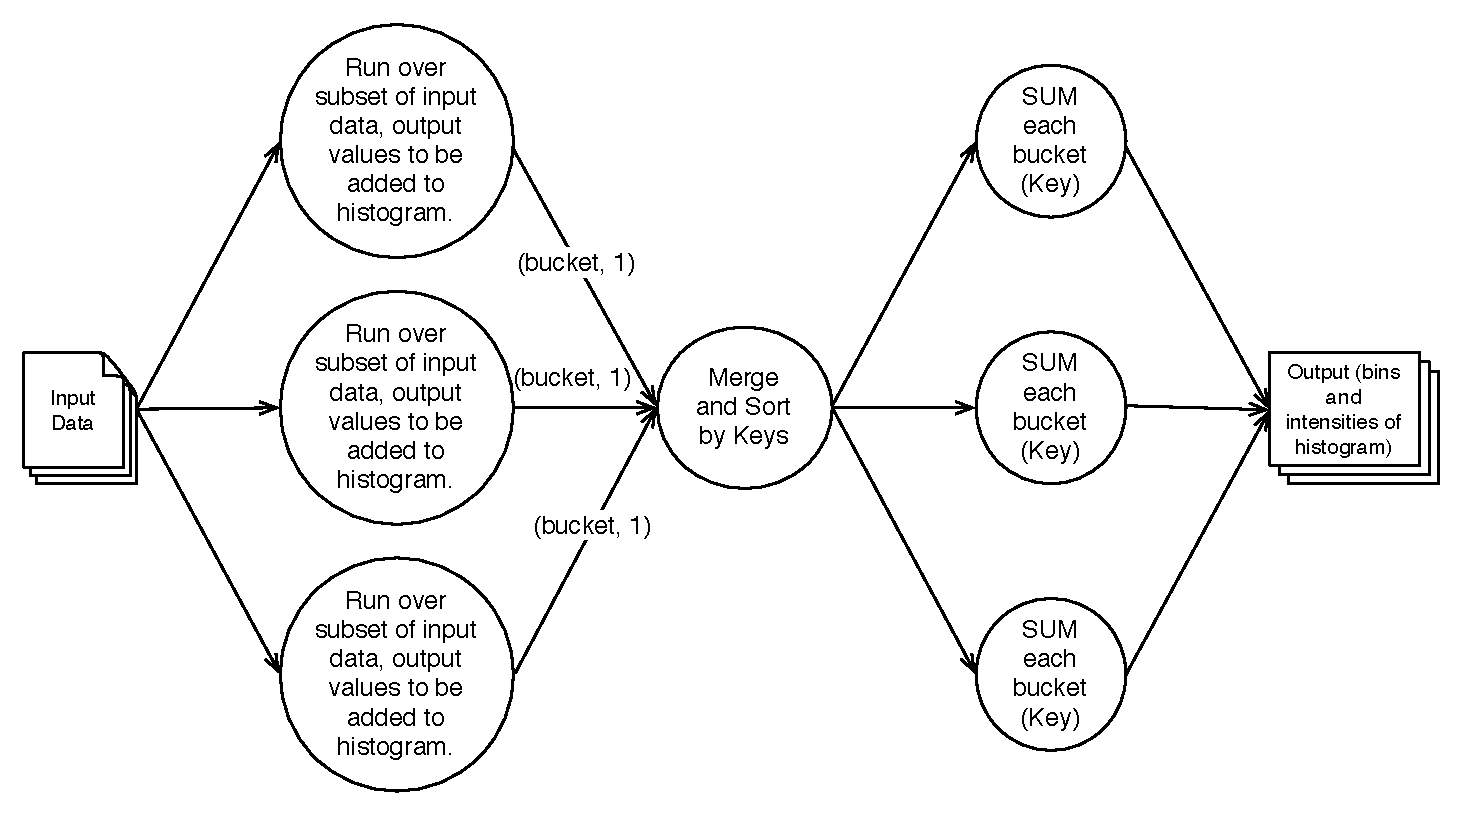
\includegraphics[width=\textwidth]{histogram-mapreduce-diag1.pdf}
\end{center}
\caption{Diagram of MapReduce Histogram Generation Pattern}
\label{fig:mr-histogram-pattern1}
\end{figure}

%\section{Application: Sending/receiving Interaction With Servers}
%
%Combined
%with an RPC system this means that one can interactively craft request
%messages, send the serialized message to a remote server, read back a
%response, and then parse the response protocol buffer interactively.

%TODO(mstokely): Talk about Jeroen Ooms OpenCPU, or talk about Andy
%Chu's Poly.


\section{Summary}

% RProtoBuf has been used.

%Its pretty useful.  Murray to see if he can get approval to talk a
%tiny bit about how much its used at Google.

%This file is only a basic article template. For full details of \emph{The R Journal} style and information on how to prepare your article for submission, see the \href{http://journal.r-project.org/latex/RJauthorguide.pdf}{Instructions for Authors}.

\section{Acknowledgement}

The first versions of \CRANpkg{RProtoBuf} were written during 2009-2010,
with very significant contributions, both in code and design, made by
Romain Fran\c{c}ois. His continued influence on design and code is
appreciated. Several features of the package are influenced
by the design of the \CRANpkg{rJava} package by Simon Urbanek
The user-defined table mechanism, implemented by Duncan Temple Lang for the
purpose of the \pkg{RObjectTables} package allowed the dynamic symbol lookup.
Kenton Varda was generous with his time in reviewing code and explaining
obscure protocol buffer semantics.  Karl Millar and Jeroen Ooms were
helpful in reviewing code or offering suggestions.  The contemporaneous
work by Saptarshi Guha on \pkg{RHIPE} was a strong initial motivator.

\bibliography{eddelbuettel-stokely}

%\section[About Java]{About \proglang{Java}}
%% Note: If there is markup in \(sub)section, then it has to be escape as above.

\end{document}
